\chapter{Linux とは}
\label{chap:what_is_linux}

% この章で学ぶこと
\begin{goalbox}
  \begin{itemize}
    \item TODO
  \end{itemize}
\end{goalbox}

\section{OS とは何か}

TODO

\section{Linux の歴史と UNIX 哲学}

TODO

\section{オープンソースソフトウェア}
\label{sec:linux-oss}

Linux カーネルは、世界中の誰でもソースコード（プログラムの設計図にあたる文字）を読むことができ、自由に改良して配ることもできます。
このように、ソースコードが公開され、誰でも利用・改良・再配布できるソフトウェアを\textbf{オープンソースソフトウェア}（Open Source Software、\textbf{OSS}）といいます。
Linux だけでなく、本書で扱う Ubuntu、Git、Python、ROS 2、Gazebo も、すべて OSS です。
ロボット開発の世界を理解するうえで、OSS の考え方は欠かせません。

\subsection{ソースコードが公開されているということ}

一般的な市販のソフトウェアは、コンピュータが実行できる形（実行ファイル）だけが配られ、ソースコードは公開されていません。
使うことはできても、中でどのような処理をしているのかを確かめたり、不具合を自分で直したりすることはできません。

これに対して OSS では、ソースコードが公開されています。
そのため、利用者は次のようなことができます。

\begin{itemize}
  \item 中身を読んで、どのように動いているのかを学ぶ
  \item 不具合を見つけたら、自分で原因を調べて直す
  \item 自分の目的に合わせて機能を追加する
  \item 改良したものを、ほかの人にも配る
\end{itemize}

ロボット開発では、センサのドライバや制御のアルゴリズムが「思ったとおりに動かない」ことがよくあります。
そのようなとき、ソースコードを読んで原因を突き止められることは、OSS の大きな強みです。

\subsection{フリーソフトウェアとオープンソース}

ソフトウェアを自由に共有しようという考え方は、1980 年代に始まった\textbf{フリーソフトウェア}運動にさかのぼります。
Richard Stallman は 1983 年に GNU プロジェクトを始め、利用者に次の 4 つの自由を保障するソフトウェアを「フリーソフトウェア」と呼びました。

\begin{enumerate}
  \item 目的を問わず、プログラムを実行する自由
  \item プログラムがどのように動いているかを調べ、改変する自由（そのためにソースコードを入手できること）
  \item コピーを再配布する自由
  \item 改変したものを配布する自由
\end{enumerate}

ここでいう「フリー」は「無料」ではなく「自由」を意味します。
その後 1998 年に、この考え方を企業などにも受け入れられやすい形で広めるため、「オープンソース」という言葉が生まれました。
2 つの言葉は重視する点が少し異なりますが、対象となるソフトウェアの多くは共通しています。

\begin{point}[OSS は「無料のソフトウェア」ではない]
  OSS の多くは無料で入手できますが、OSS の本質は価格ではなく、ソースコードを読み、改良し、共有する自由にあります。
  逆に、無料で配られていてもソースコードが公開されていないソフトウェア（フリーウェア）は OSS ではありません。
\end{point}

\subsection{ライセンス}

OSS だからといって、どのように使ってもよいわけではありません。
OSS には、利用・改変・再配布の条件を定めた\textbf{ライセンス}が付いています。
代表的なライセンスには、次のようなものがあります。

\begin{center}
  \begin{tabular}{lp{0.65\linewidth}}
    \toprule
    ライセンス & 特徴 \\
    \midrule
    GPL & 改変したものを配布するときは、同じ GPL でソースコードも公開しなければならない（Linux カーネル、Git など） \\
    MIT & 著作権表示とライセンス文を残せば、ほぼ自由に利用できる \\
    BSD & MIT とほぼ同様。著作権者の名前を宣伝に使うことを禁じるものもある \\
    Apache 2.0 & MIT に近い自由さに加え、特許の扱いを明確にしている（ROS 2、Gazebo など） \\
    \bottomrule
  \end{tabular}
\end{center}

GPL のように、改変したものにも同じ自由を引き継がせるライセンスを\textbf{コピーレフト}型、MIT や Apache 2.0 のように条件がゆるやかなライセンスを\textbf{パーミッシブ}型と呼びます。

\begin{caution}[他人のコードを使うときはライセンスを確認する]
  インターネット上で見つけたコードを自分のプログラムに取り込むときは、必ずライセンスを確認してください。
  特に、ライセンスが書かれていないコードは、公開されていても自由に使ってよいとは限りません（著作権は作者にあるため、原則として作者の許可が必要です）。
  自分でコードを公開するときも、ほかの人が安心して使えるようにライセンスを明記しましょう。
  ROS 2 のパッケージでは、\cmd{package.xml} にライセンスを書きます（\ref{chap:workspace}章）。
\end{caution}

\subsection{コミュニティによる開発}

OSS の多くは、特定の会社の中だけでなく、世界中の開発者が参加する\textbf{コミュニティ}によって開発されています。
Linux カーネルも、1991 年に Linus Torvalds が個人で公開したものが、インターネットを通じて多くの開発者の協力を得て育ってきました。
現在では、個人のボランティアだけでなく、多くの企業も開発に参加しています。

OSS の開発には、誰でも参加できます。
参加の方法は、プログラムを書くことだけではありません。

\begin{itemize}
  \item 不具合を見つけて報告する
  \item ドキュメントの誤りを直したり、翻訳したりする
  \item 使い方の質問に答える
  \item 機能を改良して、その変更を取り込んでもらうよう提案する
\end{itemize}

\begin{figure}[tb]
  \centering
  \large
  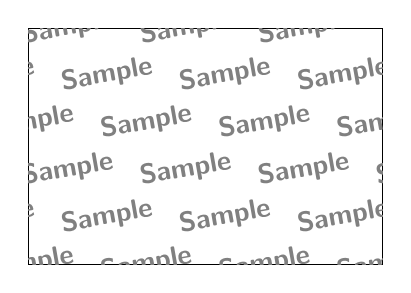
\begin{tikzpicture}
    \draw rectangle++(4.5,3);
    \clip rectangle++(4.5,3);
    \foreach\x in{0,1,2,3,4}{
      \foreach\y in{0,1,2,3,4,5,6}{
        \path(\x*1.5-\y*0.5,\y*0.6)node[rotate=10,text=gray]{\sffamily\bfseries\itshape Sample };
      }
    }
  \end{tikzpicture}
  %% 入れる画像：利用者が不具合を Issue で報告 → 開発者や利用者が修正して Pull Request → レビューを経て取り込まれ、新しい版が配布される、という循環の図
  % eps 画像を貼る場合は includegraphics をお使いください。
  % \includegraphics[width=0.8\linewidth]{ch01/oss_community.pdf}
  \caption{Issue と Pull Request による OSS 開発の流れ}
  \label{fig:linux-oss-community}
\end{figure}

こうした開発の多くは、GitHub などのサービス上で、Issue（課題の報告）や Pull Request（変更の提案）という形で行われます（\ref{chap:git}章）。
図\ref{fig:linux-oss-community}に、OSS が改良されていく流れを示します。

\subsection{ロボット開発と OSS}

ロボットを動かすには、センサからのデータの取得、地図の作成、経路の計画、モータの制御など、たくさんのソフトウェアが必要です。
これらをすべて自分たちだけで一から作るのは、現実的ではありません。

ROS は、世界中の研究者や開発者が作ったソフトウェアを OSS として共有し、組み合わせて使えるようにすることで、この問題を解決してきました。
誰かが作った地図作成のパッケージを別の誰かが改良し、それをまた別の誰かが自分のロボットで使う、という積み重ねによって、ロボット開発は大きく進歩してきたのです（\ref{chap:what_is_ros}章）。
本書の最後の\ref{chap:practice}章で体験する SLAM や自律移動も、こうした OSS の成果です。

本書を読み進めるあなたも、最初は OSS を使う側ですが、いずれは不具合の報告や改良の提案を通じて、OSS を育てる側の一員になることができます。

\begin{column}{Ubuntu と OSS のビジネス}
  「無料で配って、どうやって開発を続けているのだろう？」と疑問に思うかもしれません。
  たとえば Ubuntu は、Canonical という会社が中心となって開発しています。
  Canonical は、Ubuntu そのものは無料で配布しながら、企業向けの長期サポートやクラウド向けのサービスなどで収益を得ています。
  このように、OSS を中心にしたビジネスも数多く成り立っています。
\end{column}

\section{ディストリビューション}

TODO

\section{なぜロボット開発で Linux が使われるのか}

TODO

\section{Ubuntu 環境の用意}

TODO

\section{デスクトップ環境の基本操作}

TODO

\section*{この章のまとめ}

TODO
